%============================ Project Managenent Document ================================
% define document class
\documentclass[
	a4paper               % paper format
%	,10.5pt               % fontsize
%	,BCOR=18mm            % Binding correction
	,bibliography=totoc   % If enabled add bibliography to TOC
	,listof=totoc         % If enabled add lists to TOC
%	,bilingual
	,monolingual
	twoside=false,
]{bfhthesis}              % KOMA-script report

\setcounter{secnumdepth}{3}

\usepackage[
	hidelinks,
	pdfusetitle,
]{hyperref}
\usepackage{tikzducks}
\usepackage{amsmath}
\usepackage{hyperref}
\usepackage{listings}

\LoadBFHModule{boxes}

\colorlet{punct}{red!60!black}
\definecolor{background}{HTML}{EEEEEE}
\definecolor{delim}{RGB}{20,105,176}
\colorlet{numb}{magenta!60!black}

\lstdefinelanguage{json}{
    basicstyle=\normalfont\ttfamily,
    numbers=left,
    numberstyle=\scriptsize,
    stepnumber=1,
    numbersep=8pt,
    showstringspaces=false,
    breaklines=true,
    frame=lines,
	postbreak=\mbox{\textcolor{red}{$\hookrightarrow$}\space},
    backgroundcolor=\color{background},
    literate=
      {:}{{{\color{punct}{:}}}}{1}
      {,}{{{\color{punct}{,}}}}{1}
      {\{}{{{\color{delim}{\{}}}}{1}
      {\}}{{{\color{delim}{\}}}}}{1}
      {[}{{{\color{delim}{[}}}}{1}
      {]}{{{\color{delim}{]}}}}{1},
}

\lstdefinelanguage{canon}{
    basicstyle=\normalfont\ttfamily,
    numbers=left,
    numberstyle=\scriptsize,
    stepnumber=1,
    numbersep=8pt,
    showstringspaces=false,
    breaklines=true,
    frame=lines,
    backgroundcolor=\color{background},
	postbreak=\mbox{\textcolor{red}{$\hookrightarrow$}\space},
}

\hyphenation{ve-ri-fi-ca-tion}

\begin{document}

\frontmatter

\title{Bachelor's Thesis}
\subtitle{Unlinkability of Verfiable Credentials in a practical approach
: Project Management Document}
\author{Joël Gabriel Robles Gasser}
\institution{Bern University of Applied Sciences}
\department{Engineering and Computer Science}
\institute{Computer Science}
\version{0.1}
\advisor{Prof. Dr. Annett Laube \and Prof. Dr. Reto Koenig}
\expert{Dr. Andreas Spichiger}
\degreeprogram{Bachelor of Science in Computer Science}

%----------------  BFH tile page   -----------------------------------------
\maketitle

\addchap{Abstract}
Here an abstract might be placed.


%------------ TABLEOFCONTENTS ----------------
\tableofcontents

%------------ START MAIN PART ----------------
\mainmatter

\chapter{Introduction}
Self-sovereign Identity (SSI)\cite{self-sovereign-identity} is a concept where individuals can control their digital identity and what data is shared with whom.
In the real world physical credentials like an ID or a driver's license are used, which makes selectively disclosing information hard, as there is more information on the credentials as there is needed in one presentation.
If we digitalize these credentials, we create the option for individuals to selectively disclose information. 
Verifiable credentials (VCs)\cite{verifiable-credentials} are a type of digital credentials that can be used to represent physical credentials.
These digital credentials support multiple signing themes, one of which is the BBS Signature scheme (BBS)\cite{bbs-signature-scheme}.
This signature scheme is based on the trust triangle seen in figure \ref{fig:trusttringle}, where there are three involved parties.

\begin{figure}[h]
	\centering
	\includegraphics[width=4cm]{example-image-duck}
	\caption{The trust triangle}
	\label{fig:trusttringle}
\end{figure}

These parties are the issuer, holder and verifier.
The issuer supplies the credential to the holder, which stores it. The holder is then able to present it to a verifier, which checks its validity and content.
The verifier uses the signature to also check the authenticity and integrity of the supplied credential.
Besides signing, this signature scheme also supports proof creation, which enables unlinkability.
Unlinkability is the concept that there is no link between each credential presentation and different verifiers.
BBS also supports selective disclosure, to only disclose a subset of the information contained in the credential.\\

In this thesis we want to investigate the use of the BBS Signature Scheme in a real world scenario.
We assume that the BBS Signature scheme has no flaws, and the promoted unlinkability of the scheme holds in every situation.
We will also only use verifiable-credentials with data integrity, to not only protect the attributes of the credential (like the name, birthdate \dots) but to also protect the meta-data of the verifiable credential.
For the data integrity we will also use the BBS Signature Scheme.\\

The credentials need to send between the issuer and holder and between the holder and the verifier.
For this thesis we will only look at the messaging between the holder and the verifier and assume that the VC creation and transportation to the holder is secure.
For the presentation of the credentials there is an extension of VCs called a Verifiable-presentation (VP)\cite{verifiable-credentials}.
To present the VP we use OpenID-Connect for Verifiable-Presentations (OIDC4VP)\cite{oidc4vp}.
For OIDC4VP we assume that all communication is secured and encrypted.\\

\textit{Why not login?}
First of we would like to simply the process of a returning customer.
Think about how often you log in into Netflix, either with your email and password or with the cached login token.
It would be very unnecessary to present your VC each time you would like to watch a show, so we would like recognition.
To solve that problem we will look at Pseudonyms\cite{pseudonyms} in chapter \ref{chap:Pseudonyms}.\\

These Pseudonyms are used for a verifier to recognize already before seen individual.
This extension of the BBS Signature scheme should not break the unlinkability of the BBS proofs as they are only linkable between one verifier and the holder, but will still be analyzed.\\

Lastly we will look at the problem, where if we need to present two different VCs (like a driver's license and the vehicle registration document), how can we proof that both documents are owned by the same holder.
For that we will make use of link secrets\cite{linksecrets}, which is a secret value that only the holder knows.
% This value is supplied blinded to the issuer, meaning that is encoded in such a way that the issued cannot find out what the original value is.
% For the signer to be able to create a VC containing a blinded value, they would need to use Blind BBS Signatures\cite{bbs-signature-scheme}, which allows signing of such blinded values.
% With the blind signatures we also allow individuals to create their own credentials for their own needs, without needing to reveal the content of the credential, by using the ability to blind values.
% When a holder then presents two different credentials to a verifier, he can proof that both of those credentials are owned by him by proving the knowledge of the contents of the blinded link secrets.
In this thesis we want to analyse these concepts in conjunction with the BBS Signature scheme, to see if there is any data leakage or if the unlinkability provided by the BBS Signature Scheme will break.
For this we will investigate each concept step by step, based on their respective specifications, and implement them if needed.

\chapter{Goals}

\chapter{Recap of BLS12-381, BBS and Pairings}
This chapter contains a quick recap about BBS and BLS12-381.
The Mathematics of these topics are out of scope for this Thesis, so only the top level ideas will be discussed.

\section{BLS12-381}
\begin{figure}[h]
    \centering
	\includegraphics[width=4cm]{example-image-duck}
	\caption{The BLS12-381 curve}
	\label{fig:bls12381}
\end{figure}
The Barreto-Lynn-Scott Curves \cite{pairing-friendly-curves} are a group of pairing friendly curves. 
Specifically the BLS12-381 Curve is used in the BBS Signature Scheme \cite{bbs-signature-scheme}.
The 12 in the name comes from the embedding degree, the 381 is the amount of bits necessary to represent a point on the curve.
This Curve is defined as with the following equation $y^2 = x^3 + 4$, where x and y are coordinates on the Field $F_p$.

\subsection{Field Extensions}
$G_1$ is the largest is the largest prime order subgroup of the BLS curve.
For the Pairings discussed in section \ref{sec:pairing} we need multiple points on curves as inputs.
Besides a point on $G_1$ we also need a point on $G_2$.
This $G_2$ is an Extension of the Field $F_p$ into the Field $F_{p^2}$.
This alters the curve equation a bit to $y^2 = x^3 + 4(u + 1)$ where x and y are no longer coordinates but are polynoms of the second order.
Both $G_1$ and $G_2$ are additive Groups.
For the Pairings we also need a third Group, this time in the Field $F_{p^{12}}$.
This is Group is a multiplicative group called $G_T$ in section \ref{sec:pairing}, where x and y are polynoms of the $12^{th}$ order.
With this we now know all the necessary groups for \ref{sec:bbs}.
The Basepoints (generators) of both $G_1$ and $G_2$ are defined in \cite{pairing-friendly-curves} as follows (Big-endian order encoded as HEX):\newline

\boldmath$G_1$(BP1):\newline
x = 0x17f1d3a73197d7942695638c4fa9ac0fc3688c4f9774b905a14e3a3f171bac586c55e83ff97a1aeffb3af00adb22c6bb
y = 0x08b3f481e3aaa0f1a09e30ed741d8ae4fcf5e095d5d00af600db18cb2c04b3edd03cc744a2888ae40caa232946c5e7e1\newline\newline
\boldmath$G_2$(BP2):\newline
$x_O$ = 0x024aa2b2f08f0a91260805272dc51051c6e47ad4fa403b02b4510b647ae3d1770bac0326a805bbefd48056c8c121bdb8
$x_1$ = 0x13e02b6052719f607dacd3a088274f65596bd0d09920b61ab5da61bbdc7f5049334cf11213945d57e5ac7d055d042b7e
$y_O$ = 0x0ce5d527727d6e118cc9cdc6da2e351aadfd9baa8cbdd3a76d429a695160d12c923ac9cc3baca289e193548608b82801
$y_1$ = 0x0606c4a02ea734cc32acd2b02bc28b99cb3e287e85a763af267492ab572e99ab3f370d275cec1da1aaa9075ff05f79be

\section{BBS}
\label{sec:bbs}
\begin{figure}[h]
    \centering
	\includegraphics[width=4cm]{example-image-duck}
	\caption{The Actors of BBS and their connection}
	\label{fig:bbstriangle}
\end{figure}
The BBS Signature Scheme \cite{bbs-signature-scheme} is a multi-message signature scheme with support for selective disclosure and proof of knowledge of the signature, thus proving unlinkability between different verfiers. 
Figure \ref{fig:bbstriangle} shows the flows between the different actors.
For this thesis we define following names for the actors:
\begin{itemize}
	\item Issuer - Issues a signature on a set of messages
	\item Holder - Holds the set of messages as well as the signature. Also generates the Proof for the verifier.
	\item Verifier - Gets the disclosed messages as well as the proof, which he then verifies
\end{itemize}
For the key generation a random scalar \textbf{SK} and the Base Point of $G_2$ are needed.
Thus the public key (calculated as $SK*BP2$) results in Point on $G_2$.
This allows for all other calculations (like the signature or the proof) to be done in $G_1$ which in turn makes the algorithm more efficient.


\section{Pairings}
\label{sec:pairing}
For the verification of the BBS signature and proof Pairing-functions are used. The most important part of these functions are their billiniarity i.e.,\newline
\begin{equation}
		e(A, B + B') = e(A, B)e(A, B') \text{and} e(a * A, b * B) = e(A, B)^{ab}
\end{equation}

With these characteristics we can understand the equations for verifying the signature and proof.\newline

\textbf{Example 1. BBS Signature verification}
\begin{equation}
	\begin{split}
		Identity_{GT} & = e(A, W + BP2 * e) * e(B, -BP2) \\
		& = e(A, BP2 * e)e(A, W)e(B, BP2)^{-1} \\
		& = e(A, BP2)^ee(A, SK * BP2)e(B, BP2)^{-1} \\
		& = e(A, BP2)^ee(A, BP2)^{SK}e(B, BP2)^{-1} \\
		& = e(A, BP2)^{e + SK}e(B, BP2)^{-1} \\
		& = e(B * \frac{1}{sk * e}, BP2)^{e + SK}e(B, BP2)^{-1} \\
		& = e(B, BP2)^{\frac{e + SK}{e + SK}}e(B, BP2)^{-1} \\
		& = e(B, BP2)^1e(B, BP2)^{-1} \\
		& = e(B, BP2)^0 \\
		& = 1
	\end{split}
\end{equation}

\chapter{Use Cases}
For this Thesis we will use a small collection of use cases to demonstrate how BBS should work in conjunction with extensions (like VC's, Link Secrets etc.).

\section{Simply buying a train and mobile subscription}
Lets assume you want to go and buy a train subscription.
Once at the counter, the employee ask you for your ID card, to verify your identity and to get the required data for the subscription.
Now the employee should only need to check if the ID is valid, if the photo on it matches you, something to link your subscription to you (your name is used for that most of the time) and maybe he also needs your birthday for an age specific discount.
By handing out your ID, you lose the ability to selectively disclose information about yourself, and with that you lose your anonymity.


\begin{figure}[h]
	\begin{minipage}{0.28\textwidth}
		\textbf{Client}\newline\newline
		
\begin{tikzpicture}
			\duck[graduate]
		\end{tikzpicture}
	\end{minipage}\hfill
	\begin{minipage}{0.28\textwidth}
		$$\underrightarrow{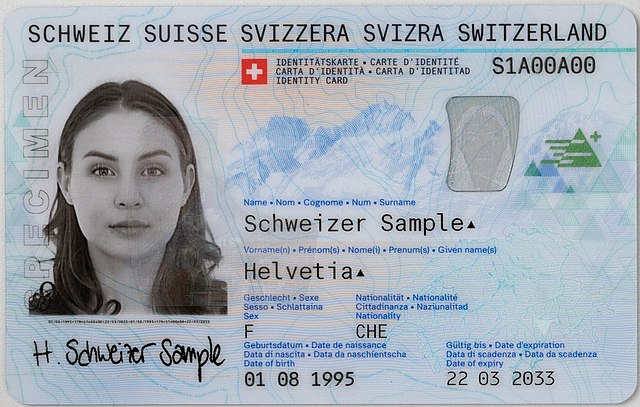
\includegraphics[width=30mm]{./img/ID.jpg}}$$
		$$\overleftarrow{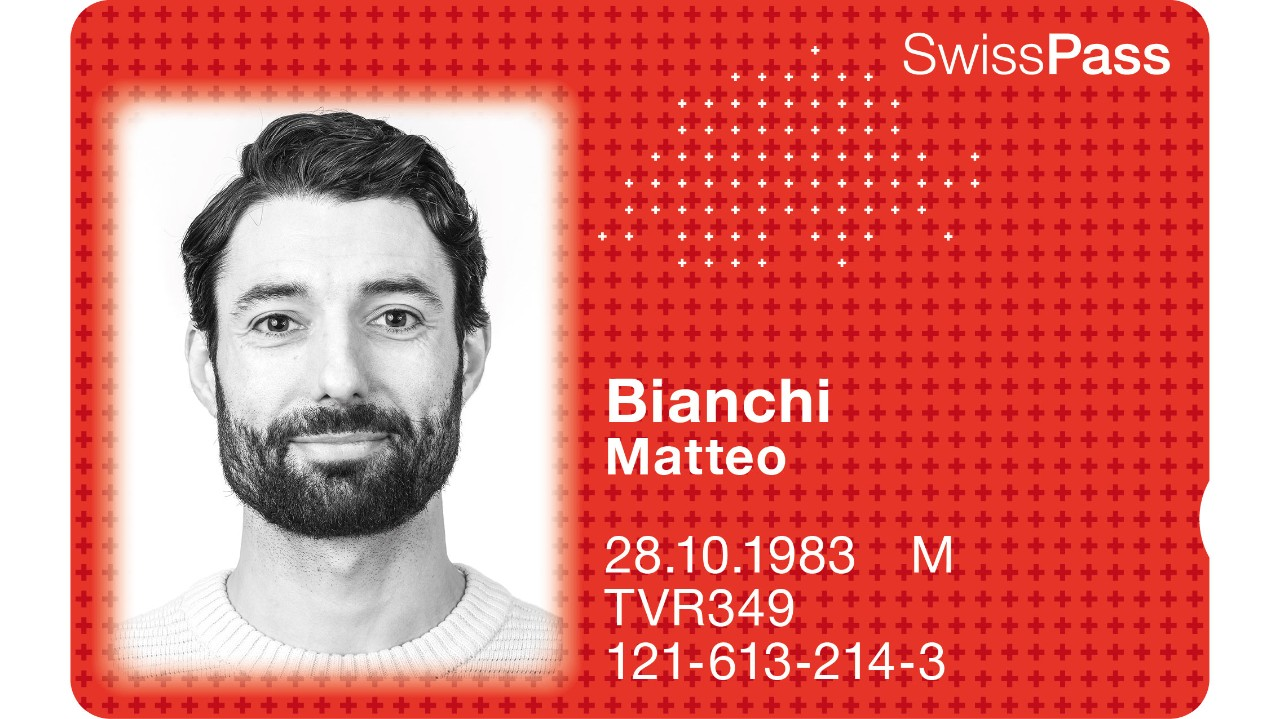
\includegraphics[width=30mm]{./img/Swisspass.jpeg}}$$
	\end{minipage}\hfill
	\begin{minipage}{0.28\textwidth}
		\textbf{SBB}\newline\newline
		
\begin{tikzpicture}
			\duck[tshirt, jacket=blue!50!black, tie=red]
		\end{tikzpicture}
	\end{minipage}
	\caption{Buying a train subscription}
	\label{fig:trainsub}
\end{figure}

Now you also need a mobile subscription. You go to your next Swiss Post office.

\begin{figure}[h]
	\begin{minipage}{0.28\textwidth}
		\textbf{Client}\newline\newline
		
\begin{tikzpicture}
			\duck[graduate]
		\end{tikzpicture}
	\end{minipage}\hfill

	\begin{minipage}{0.28\textwidth}
		$$\underrightarrow{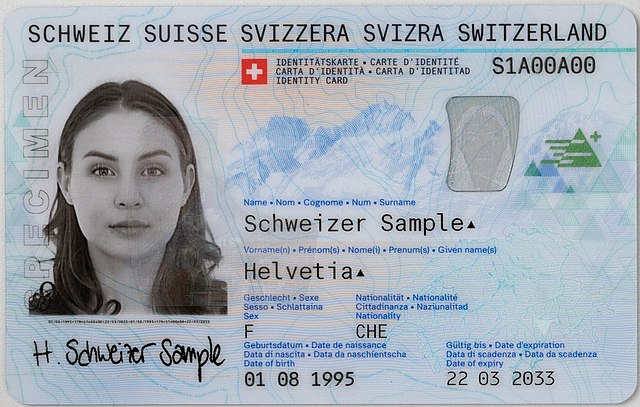
\includegraphics[width=30mm]{./img/ID.jpg}}$$
		$$\overleftarrow{\includegraphics[width=30mm]{example-image-duck}}$$
	\end{minipage}\hfill

	\begin{minipage}{0.28\textwidth}
		\textbf{Swiss Post}\newline\newline
		
\begin{tikzpicture}
			\duck[tshirt, jacket=yellow!50!orange, tie=black]
		\end{tikzpicture}
	\end{minipage}
	
	\caption{Buying a mobile subscription}
	\label{fig:mobilesub}
\end{figure}

Here, the employee makes the same checks as the SBB employee to see if you are who you say you are.
And again, by handing out your ID, you lose the ability to selectively disclose information about yourself.

\begin{figure}
	\includegraphics[width=30mm]{example-image-duck}
\end{figure}

Now lets say but verifiers collude. As they have the same information about you, they link it back to you and create a profile about.
In \autoref{chap:bbsex} we will see how we can use BBS to restore unlinkability and more.

\chapter{Extensions with BBS}
\label{chap:bbsex}

\section{BBS with VC's}
The BBS signatures and proofs as well as the messages need to be transported somehow.
For this Thesis we chose Verifiable credentials \cite{verifiable-credentials} as the representation of these attributes.
But what are VC's? \newline
Verifiable credentials are JSON-LD data models, designed to represent different types of digital credentials.
The Idea, is to be able to translate physical credentials, like an ID or a driver's license, into the digital world.
In this Thesis we will only look at a small part of the standard, just enough that we can use it together with BBS.
We will also use VPs, or Verifiable Presentations. These are praticly a VC wrapped in an other VC.
A concrete example can be found in chapter \dots
All VC concepts described can also be applied to VPs, so VP and VC can be used interchangeably.

\subsection{Used VC concepts}
In this section we will define which VC concepts are used in this thesis.

\subsubsection{@context}
The \textbf{@context} attribute are used to map human-friendly ids like \textit{type} to an url.
These urls then help the system understand what the content of the VC is.
The value of the \textbf{@context} attribute is an ordered list, where the first entry must be \verb|<https://www.w3.org/ns/credentials/v2>|
We will also use the context \verb|<https://w3id.org/security/data-integrity/v2>| to signify that the content of the VC is protected.
Lastly we use a custom context, which describes the content in the credentialSubject.

Our custom context looks like this:
\begin{lstlisting}[language=json,firstnumber=1,caption={Example custom context},captionpos=b]
{
    "@context":{
        "first_name": "https://schema.org/givenName",
        "last_name": "https://schema.org/familyName"
    }
}
\end{lstlisting}

The complete \textbf{@context} which we will use in our example, where the different contexts are represented by urls, looks like this:
\begin{lstlisting}[language=json,firstnumber=1,caption={Example context},captionpos=b]
{
	"@context": [
		"https://www.w3.org/ns/credentials/v2",
		"https://w3id.org/security/data-integrity/v2",
		"https://raw.githubusercontent.com/RockstaYT/BA_Thesis_BBS_Signatures/docs/context/example_1.jsonld"
	],
}
\end{lstlisting}

\subsubsection{id}

TODO: Will be looked at later with the ZKP \& revocation

\subsubsection{type}

The \textbf{type} defines what the VC is. 
It is a set containing either urls to the description of the VC or be an ID that can be mapped through \textbf{@context}.
If we use the standard mapped IDs, the type set must either include \textit{VerifiableCredential} or \textit{VerifiablePresentation}.
If we want, we can also add a more specific type, in which we define more information about the VC.

May be used later \dots

\subsubsection{credentialSubject}
The credentialSubject contains a set of objects, which each contain multiple statements about the subject of the credential.
In our first example we only have one object with two statements about the subject, namely \textit{first\_name} and \textit{last\_name}.

Such a credential subject may look like this:
\begin{lstlisting}[language=json,firstnumber=1,caption={Example credentialSubject},captionpos=b]
{
	"credentialSubject":{
		"first_name": "Joel",
		"last_name": "Robles"
	}
}
\end{lstlisting}

\subsubsection{proof}

proof = signature, but also = proof, depending on VC or VP.

\subsection{Prepare VCs for BBS and sign them}
\label{sub:preparevc}
Now that we know the different concepts that we use for the example, we can look into how to prepare the VC to be signed by the BBS signature scheme.
VCs are JSON objects with multiple key-value pairs on different levels, while BBS can only sign statements.
So somehow we need to transform the JSON object into statements, which then can be signed by BBS.
To achieve this we will use the \textit{Data Integrity BBS Cryptosuites draft}\cite{bbsvc}.

We will be using the following VC as an example.
\begin{lstlisting}[language=json,firstnumber=1,caption={Example VC},captionpos=b]
{
	"@context": [
		"https://www.w3.org/ns/credentials/v2",
		"https://w3id.org/security/data-integrity/v2",
		"https://raw.githubusercontent.com/RockstaYT/BA_Thesis_BBS_Signatures/docs/context/example_1.jsonld"
	],
	"type":  ["VerifiableCredential"],
	"credentialSubject":{
		"first_name": "Joel",
		"last_name": "Robles"
	}
}
\end{lstlisting}

We define following variables:\newline
\textbf{vc}: The VC document\newline
\textbf{hmac\_key}: A 32-bit random string, which is later used to initialize an HMAC.\newline
\textbf{verification\_method}: The url to the verification method\\
\textbf{mandatory\_attributes}: A set of attributes which are mandatory for the holder to disclose to the verifier. For this example we will set the \textit{first\_name} as mandatory. This may look like this: ["credentialSubject/first\_name"].\newline

Now follow these steps to transform and sign the VC:
\begin{itemize}
	\item Set \textbf{proof\_config} and \textbf{canonical\_proof\_config} to the respective entry in the result of the algorithm described in chapter \ref{subsubsec:proof_config} with the inputs \textbf{vc.@context} and \textbf{verification\_method}
	\item Set \textbf{transformed\_document} to the result of the algorithm described in chapter \ref{chap:transform} with the inputs \textbf{vc}, \textbf{mandatory\_attributes} and \textbf{hmac\_key}.
	\item Set \textbf{hash\_data} to the result of the algorithm described in chapter \ref{subsubsec:proofHash} with the inputs \textbf{canonical\_proof\_config}, \textbf{mandatory\_attributes} and \textbf{transformed\_document}
	\item Set \textbf{base\_proof} to the result of the algorithm described in chapter \ref{subsubsec:sign} with the inputs \textbf{hash\_data} and \textbf{mandatory\_attributes}.
	\item Set \textbf{signed\_vc} to the result of the algorithm described in chapter \ref{subsubsec:signed} with the inputs \textbf{vc}, \textbf{proof\_config} and \textbf{base\_proof}.
\end{itemize}

And with that \textbf{signed\_vc} is a valid signed VC, that can be used to generate a derived VP with selective disclosure and unlinkable proofs.

This VC may look like this:

\begin{lstlisting}[language=json,firstnumber=1,caption={Signed VC},captionpos=b]
{
	"@context": [
		"https://www.w3.org/ns/credentials/v2"
	],
	"type": [
		"VerifiableCredential"
	],
	"credentialSubject": {
		"first_name": "Joel",
		"last_name": "Robles"
	},
	"proof": {
		"type": "DataIntegrityProof",
		"cryptosuite": "bbs-2023",
		"created": "2024-04-03T22:11:27.027Z",
		"verificationMethod": "did:key:zUC7DerdEmfZ8f4pFajXgGwJoMkV1ofMTmEG5UoNvnWiPiLuGKNeqgRpLH2TV4Xe5mJ2cXV76gRN7LFQwapF1VFu6x2yrr5ci1mXqC1WNUrnHnLgvfZfMH7h6xP6qsf9EKRQrPQ#zUC7DerdEmfZ8f4pFajXgGwJoMkV1ofMTmEG5UoNvnWiPiLuGKNeqgRpLH2TV4Xe5mJ2cXV76gRN7LFQwapF1VFu6x2yrr5ci1mXqC1WNUrnHnLgvfZfMH7h6xP6qsf9EKRQrPQ",
		"proofPurpose": "assertionMethod",
		"proofValue": "u2V0ChdhAWFC2HFadcICoWHnR-s9oPaUegpsXqwH_8ngk4TBuMLDFqnvVCo9axh2gcmb2w4KJ5LlfQOgl6M_YY3waJwFPMF5oqtZGI0rzf6HfWOS6VfGPWthAWEClRFA4ut1V3aj4gUvaZAvy2PvZHn-CFZzt5TUfXODzG0MDCe45ZPrMkpKH4UaaxIUqC6L_lhaGZLEMu5ae3gHb2EBYYKTvGvo9pXVJbxIrm3i4wkdhUxqKCTIGrnxFuAdZwWi6T3omD5wzZ7bAGbRneEEQSxBmXtvnC6Pr59nPv_v3HrAW9wq_uxYzF_NyaX3GPv0h_FV2T2OSao8C6uoyWiqIj9hAWCAAESIzRFVmd4iZqrvM3e7_ABEiM0RVZneImaq7zN3u_4F4HS9jcmVkZW50aWFsU3ViamVjdC9maXJzdF9uYW1l"
	}
}
\end{lstlisting}

\subsubsection{Shuffled label map}
\label{sub:shuffledlabelmap}

Because of security considerations mentioned in chapter \ref{subsec:vcseccons} the canonicalised \textbf{vc} needs to be shuffled.

The required inputs of this algorithm is random 32-bit long bit-string named \textbf{hmac\_key} which will be used to initialize a \textit{HMAC}.

The output is a function called \textbf{label\_map\_factory\_function}.

% We also need a map of the canonical ids named \textbf{canonical\_id\_map}, where the node prefixes \textbf{\_:} are stripped (from \textit{\_:c14n0} to \textit{c14n0}).
% This map may look like this:
% \begin{lstlisting}[language=canon,firstnumber=1,caption={Example canonical id map},captionpos=b]
% [
%   "_:_e3e2ad71-3a6d-4b66-8f57-b3ae79f6dcad_1",
%   "_:c14n0",
% ]
% \end{lstlisting}

% The output is a bnode map named \textbf{bnode\_id\_map}, which may look like this:
% \begin{lstlisting}[language=canon,firstnumber=1,caption={Example canonical id map},captionpos=b]
% [
% 	"_e3e2ad71-3a6d-4b66-8f57-b3ae79f6dcad_1",
% 	"b1",
% ]
% \end{lstlisting}

% As you can see the canonical id \textit{\_:c14n0} is replaced with a bnode id \textit{b1}.

% The return of this algorithm is a bnode id map named \textbf{bnode\_id\_map}

\begin{itemize}
	\item Create a function with the name \textbf{label\_map\_factory\_function}, which has one required input named \textbf{canonical\_id\_map}. Inside the function do these steps:
	\begin{itemize}
		\item Initialize \textbf{bnode\_id\_map} to a new map.
		\item For each entry in the \textbf{canonical\_id\_map}, which are split up into key - value
		\begin{itemize}
			\item Set \textbf{hmac\_result} to result of a HMAC-digest operation, which was initialized with the \textbf{hmac\_key}, on the value of the entry. 
			\item Add a new map entry into \textbf{bnode\_id\_map}, where the key is the key from \textbf{canonical\_id\_map} and the value is \textbf{hmac\_result} encoded in base64-url encoding defined in chapter 5 and 3.2 of "RFC 4648"\cite{base64}.
		\end{itemize}
		\item Initialize \textbf{hmac\_ids} to the sorted values of \textbf{bnode\_id\_map}
		\item For each key in the \textbf{bnode\_id\_map}
		\begin{itemize}
			\item Set the value for the given key in \textbf{bnode\_id\_map} with \textbf{b} concatenated with the index of the correspoing value in \textbf{hmac\_ids}. The value should then look like \textbf{b0}.
		\end{itemize}
		\item Finally return \textbf{bnode\_id\_map}.
	\end{itemize}
	\item Return \textbf{label\_map\_factory\_function}
\end{itemize}

\subsubsection{Create the proof config}
\label{subsubsec:proof_config}
The proof config contains the information about the proof to be generated, like what cryptosuite was used, what type of proof it is \dots

The required inputs of this algorithm are the url of the verification information \textbf{verification\_method} and the context of the VC \textbf{@context}.

The output of this algorithm is the proof config \textbf{proof\_config} and the canonicalised proof config \textbf{canonical\_proof\_config}.

\begin{itemize}
	\item Create an empty \textbf{proof\_config} object
	\item Set \textbf{proof\_config.type} to \textit{DataIntegrityProof}
	\item Set \textbf{proof\_config.cryptosuite} to \textit{bbs-2023}
	\item Set \textbf{proof\_config.created} to the current time
	\item Set \textbf{proof\_config.verificationMethod} to the url of the verification information \textbf{verification\_method} (see: \url{https://www.w3.org/TR/vc-di-bbs/#multikey})
	\item Set \textbf{proof\_config.@context} to \textbf{@context}
	\item Set \textbf{canonical\_proof\_config} to the canonical representation of the \textbf{proof\_config} using the \textit{Universal RDF Dataset Canonicalization Algorithm}\cite{rdf}
	\item Return an object containing \textbf{proof\_config} and \textbf{canonical\_proof\_config}.
\end{itemize}

If we follow the instructions step by step we get a JSON object like this:
\begin{lstlisting}[language=json,firstnumber=1,caption={Example Proof Config},captionpos=b]
{
	"type": "DataIntegrityProof",
	"cryptosuite": "bbs-2023",
	"created": "2024-04-01T21:28:52.401Z",
	"verificationMethod": "www.example.com/keys",
	"proofPurpose": "assertionMethod",
	"@context": [
		"https://www.w3.org/ns/credentials/v2"
	],
}
\end{lstlisting}

Which in turn is canonicalised into this:

\begin{lstlisting}[language=canon,firstnumber=1,caption={Example Proof Config canonicalized},captionpos=b]
_:c14n0 <http://purl.org/dc/terms/created> "2024-04-01T21:35:10.679Z"^^<http://www.w3.org/2001/XMLSchema\#dateTime> .
_:c14n0 <http://www.w3.org/1999/02/22-rdf-syntax-ns\#type> <https://w3id.org/security\#DataIntegrityProof> .
_:c14n0 <https://w3id.org/security\#cryptosuite> "bbs-2023"^^<https://w3id.org/security\#cryptosuiteString> .
_:c14n0 <https://w3id.org/security\#proofPurpose> <https://w3id.org/security\#assertionMethod> .
_:c14n0 <https://w3id.org/security\#verificationMethod> <did:key:zUC7DerdEmfZ8f4pFajXgGwJoMkV1ofMTmEG5UoNvnWiPiLuGKNeqgRpLH2TV4Xe5mJ2cXV76gRN7LFQwapF1VFu6x2yrr5ci1mXqC1WNUrnHnLgvfZfMH7h6xP6qsf9EKRQrPQ\#zUC7DerdEmfZ8f4pFajXgGwJoMkV1ofMTmEG5UoNvnWiPiLuGKNeqgRpLH2TV4Xe5mJ2cXV76gRN7LFQwapF1VFu6x2yrr5ci1mXqC1WNUrnHnLgvfZfMH7h6xP6qsf9EKRQrPQ> .
\end{lstlisting}

With that we have our \textbf{canonical\_proof\_config} and the first step is finished.

\subsubsection{Transform the VC}
\label{chap:transform}
This algorithm transforms VC into statements which can later be signed by bbs.

The required inputs are a VC document \textbf{vc}, a 32-byte long \textbf{hmac\_key} to initialize a HMAC and a set of mandatory pointers \textbf{mandatory\_attributes}.

\begin{itemize}
	\item Define \textbf{label\_map\_factory\_function} as the function which is returned from the \textbf{create\_shuffled\_id\_label\_map\_function} defined in chapter \ref{sub:shuffledlabelmap} with the input \textbf{hmac\_key}.
	\item Set \textbf{group\_definitions} to a map where \textit{mandatory} is the key and the value is \textbf{mandatory\_attributes}.
	\item Set \textbf{groups} to the \textit{response.groups} of the \textit{canonicalizeAndGroup} algorithm specified in the DataIntegrity for ECDSA specification\cite{ecdsa}, passing the \textbf{label\_map\_factory\_function}, \textbf{group\_definitions} and \textbf{vc}.
	\item Set \textbf{mandatory} to the value from \textbf{groups.mandatory.matching}
	\item Set \textbf{nonMandatory} to the value from \textbf{groups.mandatory.nonMatching}
	\item Return an object named \textbf{transformed\_data} containing \textit{mandatory} set to \textbf{mandatory}, \textit{nonMandatory} set to \textbf{nonMandatory} and \textit{hmacKey} set to \textbf{hmacKey}.
\end{itemize}

This object may look like this:

\begin{lstlisting}[language=json,firstnumber=1,caption={Return object of the VC transformation},captionpos=b]
{
	"mandatory": [[
		0,
		"_:b0 <https://www.w3.org/ns/credentials/issuer-dependent#first_name> \"Joel\" .\n",
		],
		[
		2,
		"_:b1 <http://www.w3.org/1999/02/22-rdf-syntax-ns#type> <https://www.w3.org/2018/credentials#VerifiableCredential> .\n",
		],
		[
		3,
		"_:b1 <https://www.w3.org/2018/credentials#credentialSubject> _:b0 .\n",
		]],
	"nonMandatory": [[
		1,
		"_:b0 <https://www.w3.org/ns/credentials/issuer-dependent#last_name> \"Robles\" .\n",
	  ]],
	"hmacKey": [0, 17, 34, 51, 68, 85, 102, 119, 136, 153, 170, 187, 204, 221, 238, 255, 0, 17, 34, 51, 68, 85, 102, 119, 136, 153, 170, 187, 204, 221, 238, 255],
}
\end{lstlisting}

And with that we transformed the VC into canonical statements that can later be signed by BBS.

\subsubsection{Hash the proof data}
\label{subsubsec:proofHash}
This algorithm creates a hash of the proof data, which will be used as the header of for the bbs signature operation.

The input for this algorithm is the proof config as canonical staments \textbf{canonical\_proof\_config}, a set of mandatory pointers \textbf{mandatory\_attributes} and a transformed document \textbf{transformed\_data}

The output is an object \textbf{hash\_data} which is a copy of the \textbf{transformed\_data} with new key-value pairs.


\begin{itemize}
	\item Set \textbf{proof\_hash} as the result of the hashing of \textbf{canonical\_proof\_config} using SHA-256.
	\item Set the \textbf{mandatory\_hash} as the result of the hashing of \textbf{transformed\_document.mandatory} using SHA-256. Be aware that mandatory is an array that first needs to be concatenated. In this thesis we don't use any delimiter for concatenation.
	\item Initialise \textbf{hash\_data} as a copy of \textbf{transformed\_data}, then adding the key-value pairs \textit{proofHash} - \textbf{proof\_hash} and \textit{mandatoryHash} - \textbf{mandatory\_hash}
	\item Return \textbf{hash\_data}
\end{itemize}

With this object we now have all data to be able to create a bbs signature.

\subsubsection{Generate and serialize the signature}
\label{subsubsec:sign}
This algorithm shows how the different data prepared in the algorithms before, is used to generate a valid bbs signature.

The inputs for this algorithm are the hashed proof data \textbf{hash\_data} and a set of mandatory pointers \textbf{mandatory\_attributes}.

\begin{itemize}
	\item Set \textbf{proof\_hash}, \textbf{mandatory\_hash}, \textbf{non\_mandatory} and \textbf{hmac\_key} to the corresponding value in \textbf{hash\_data}.
	\item Set \textbf{bbs\_header} to the concatenation of \textbf{proof\_hash} and \textbf{mandatory\_hash}
	\item Set \textbf{bbs\_messages} to the messages in the \textbf{non\_mandatory} array, which are represented as byte arrays encoded with UTF-8
	\item Set \textbf{bbs\_signature} to the result of the bbs signature operation, defined in chapter 3.5.1 of the BBS Siganture Scheme\cite{bbs-signature-scheme}.
	\item Initialise \textbf{proof\_value} to the bbs proof header bytes 0xd9, 0x5d and 0x02
	\item Set \textbf{components} to an array containing(in this order): \textbf{bbs\_signature}, \textbf{bbs\_header}, \textbf{public\_key}, \textbf{hmac\_key}, \textbf{mandatory\_pointers}
	\item Set \textbf{cbor} to result of the application of the CBOR-encoding\cite{cbor}, where CBOR tagging \textbf{Must NOT} be used.
	\item Set \textbf{proof\_value} to the concatenation of \textbf{proof\_value} and \textbf{cbor}
	\item Set \textbf{base\_proof} to the value of the base64-url encoding defined in chapter 5 of "RFC 4648"\cite{base64} but without padding as mentioned in chapter 3.2 of the same RFC.
	\item Return \textbf{base\_proof}
\end{itemize}

We now have a valid bbs signature, which we can append to the VC.

\subsubsection{Add signature to VC}
\label{subsubsec:signed}
This algorithm adds a bbs signature to a VC document.

The input to this algorithm is a VC \textbf{vc}, the base proof \textbf{base\_proof} and a proof config \textbf{proof\_config}.

The output of this algorithm is a signed VC with the proof information attached.

\begin{itemize}
	\item Add a new key-value pair \textit{proof} - \textbf{proof\_config} to \textbf{vc}
	\item Add a new key-value pair \textit{proofValue} - \textbf{base\_proof} to \textbf{vc.proof}
	\item Return \textbf{vc}
\end{itemize}

And with that we now have a fully functional VC which was signed with bbs.

\subsection{Derive selective disclosure VPs}
As a holder of a secured VC, one would like to present that VC to a verifier.
For that we create a Verifiable Presentation (VP), which in turn is just a VC containing \textit{@context}, \textit{type} and the VC as \textit{verifiableCredential}.
We also want to use the selective disclosure provided by the bbs signature scheme, so that we don't need to disclose all the information contained in the VC.
For that we use the algorithm described in chapter \ref{subsub:derivevp}.
We will use the same example as in chapter \ref{sub:preparevc}.
As in that example we forced the disclosure of the \textit{last\_name} we will define that no more information should be revealed, meaning that the \textit{first\_name} will not be revealed to the verfier.\\

We define following variables:\\
\textbf{vc}: The VC, \textbf{not containing} the proof object\\
\textbf{selective\_pointers}: A array containing pointers on what should be revealed. As already mentioned, in this example we will not reveal anything, so this variable is an empty array [].\\
\textbf{ph}: The presentation header as a byte array. We will define it as an empty array [] for this example.\\

\subsubsection{Derive VP}
\label{subsub:derivevp}


\subsubsection{Create disclosure data}
\label{subsub:createdisclosuredata}

This algorithm creates the data for the selective disclosure of a VP.
The inputs of this algorithm are a VC \textbf{vc}, the proof \textbf{base\_proof}, the selective pointers \textbf{selective\_pointers} and a presentation header \textbf{ph}.
The output is \dots

We follow these steps:
\begin{itemize}
	\item Set \textbf{bbs\_signature}, \textbf{bbs\_header}, \textbf{public\_key}, \textbf{hmac\_key} and \textbf{mandatory\_pointers} to their respective value in the response of the algorithm described in chapter \ref{subsub:parsebaseproof}
	\item Define \textbf{label\_map\_factory\_function} as the function which is returned from the \textbf{create\_shuffled\_id\_label\_map\_function} defined in chapter \ref{sub:shuffledlabelmap} with the input \textbf{hmac\_key}
	\item Set \textbf{combined\_pointers} to the concatenation of \textbf{mandatory\_pointers} and \textbf{selective\_pointers}
	\item Set \textbf{group\_definitions} to an object with following key-value pairs: \textit{mandatory} - \textbf{mandatory\_pointers}, \textit{selective} - \textbf{selective\_pointers} and \textit{combined} - \textit{combined\_pointers}
	\item Set \textbf{groups} and \textbf{label\_map} to \textit{response.groups} and \textit{response.labelMap} respectively of the \textit{canonicalizeAndGroup} algorithm specified in the DataIntegrity for ECDSA specification\cite{ecdsa}, passing the \textbf{label\_map\_factory\_function}, \textbf{group\_definitions} and \textbf{vc}.
	\item Set \textbf{combined\_match} to \textbf{groups.combined.matching}
	\item Set \textbf{mandatory\_match} to \textbf{groups.mandatory.matching}
	\item Set \textbf{combined\_indexes} to the ordered list of \textbf{combined\_match.keys}
	\item Set \textbf{mandatory\_indexes} to an empty array. We want to compute the position of the mandatory indexes in the \textbf{combined\_match} array, so that the verifier knows which indexes were mandatory to reveal
	\item For each key in \textbf{mandatory\_match} find its index in \textbf{combined\_indexes} and add it to \textbf{mandatory\_indexes}.
	\item Set \textbf{selective\_match} to \textbf{groups.selective.matching}
	\item Set \textbf{mandatory\_non\_match} to \textbf{groups.mandatory.nonMatching}
	\item Set \textbf{non\_mandatory\_indexes} to the ordered list of \textbf{mandatory\_non\_match.keys}
	\item Set \textbf{selective\_indexes} to an empty array. This time we want to compute the position of the selective indexes in the \textbf{non\_mandatory\_indexes} list. This list will be used for the bbs proof generation process, to define which messages are going to be revealed.
	\item For each key in \textbf{selective\_match} find its index in \textbf{non\_mandatory\_indexes} and add it to \textbf{selective\_indexes}
	\item Set \textbf{bbs\_messages} to the values of \textbf{non\_mandatory.values} as byte arrays
	\item Set \textbf{bbs\_proof} to the result of the bbs proof operation defined in chapter 3.5.3 of \textit{The BBS Signature Scheme}\cite{bbs-signature-scheme}, with the input \textbf{public\_key}, \textbf{bbs\_signature}, \textbf{bbs\_header}, \textbf{ph}, \textbf{bbs\_messages} and \textbf{selective\_indexes}
	\item Set \textbf{initial\_document} to the result of the algorithm described in chapter 3.4.13 of \textit{Data Integrity ECDSA Cryptosuites v1.0}\cite{ecdsa}, with the inputs \textbf{vc} and \textbf{combined\_pointers}
	\item 
\end{itemize}


\subsubsection{Parse the base proof}
\label{subsub:parsebaseproof}

This algorithm parses a base proof value back to objects.
The input of this algorithm is a base proof \textbf{base\_proof}.
The output is a object \textbf{parsed\_base\_proof} containing the parsed base proof values.

We follow these steps to parse the base proof:
\begin{itemize}
	\item Check that the \textbf{base\_proof} start with a \textit{u}, indicating that it is a base64-url encoded string.
	\item Set \textbf{decoded\_proof\_value} to the result of the base64-url decoding with no padding as described in \textit{The Base16, Base32, and Base64 Data Encodings}\cite{base64}
	\item Check that \textbf{decoded\_proof\_value} starts with the proof header bytes \textit{0xd9}, \textit{0x5d} and \textit{0x02}
	\item Set \textbf{components} to the cbor decoding described in \textit{RFC 8949}\cite{cbor}, starting with the fourth byte in \textbf{decoded\_proof\_value}
	\item Set \textbf{base\_proof\_object} to the key-value pairs \textit{bbs\_signature} - \textbf{components[0]}, \textit{bbs\_header} - \textbf{components[1]}, \textit{public\_key} - \textbf{components[2]}, \textit{hmac\_key} - \textbf{components[3]} and \textit{mandatory\_pointers} - \textbf{components[4]}
	\item Return \textbf{base\_proof\_object}
\end{itemize}

With that we parsed the base proof bytes back to objects.


\subsection{Security Considerations of VCs}
\label{subsec:vcseccons}

\section{BBS with Pseudonyms}
\label{chap:Pseudonyms}

\section{BBS with Link Secrets}
\label{chap:linksecrets}

\section{BBS with Blind Signatures}
\label{chap:blindsignatures}




\appendix


\chapter{First appendix Chapter}



\bibliographystyle{plain}
\bibliography{refs}

\end{document}
